
%%%%%%%%%%%%%%%%%%%%%%%%%%%%%%%%%%%%%%%%%%%%%%%%%%%%%%%%%%%
\section{Experiment}\label{sec:expResults}
%%%%%%%%%%%%%%%%%%%%%%%%%%%%%%%%%%%%%%%%%%%%%%%%%%%%%%%%%%%



\subsection{Hardware system}


Our experiments are on centimeter-scale hardware systems called \emph{kilobots}.  These allows us to emulate a variety of dynamics, while enabling a high degree of control over robot function, the environment, and data collection. The kilobot \cite{Rubenstein2012,rubenstein2014programmable} is a low-cost robot designed for testing collective algorithms with large numbers of robots. It is available commercially or as an open source platform~\cite{K-Team2015}.  Each robot is approximately 3 cm in diameter, 3 cm tall, and uses two vibration motors to move on a flat surface at speeds up to 1 cm/s.  Each robot has one ambient light sensor that is used to implement \emph{phototaxis},  moving towards a light source. 
In these experiments as shown in Fig.~\ref{fig:setup} , we used $n$=64 kilobots, a 1.5 m$\times$1.2 m whiteboard as the workspace, and four 30W LED floodlights arranged 1.5 m above the plane of the table at the $\{N,E,S,W\}$ vertices of a 6 m square centered on the workspace. The lights were controlled using an Arduino Uno board connected to an 8 relay shield board.  At top of the table, an overhead machine vision system was added to track the position of the swarm. Laser-cut patterns for our neon green fiducial markers and our {\sc Matlab} tracking code are available at our github repository~\cite{Shahrokhi2015GitHubShapeControl}.


\begin{figure}
\begin{center}
	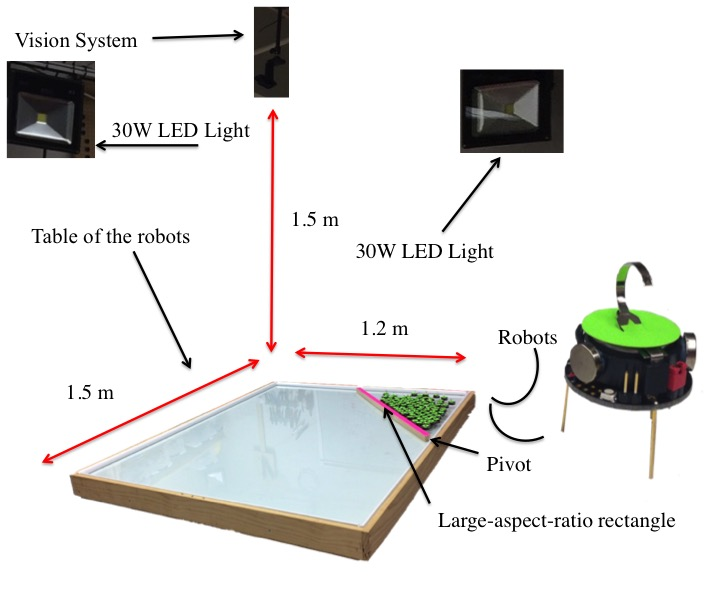
\includegraphics[width=\columnwidth]{SetUp.jpg}
\end{center}
\caption{\label{fig:setup}
Hardware platform:  table with 1.5$\times$1.2 m workspace, surrounded by four remotely triggered 30W LED floodlights, with an overhead machine vision system.
}
\end{figure}

The walls of the hardware platform have almost infinite friction, due to the three legged design of the kilobots. When a kilobot is steered into the wall, they pin themselves to the wall until the light changes direction and they begin turning in the other direction.  This wall friction is sufficient to enable independent position control of two kilobots, as shown in Fig.~\ref{fig:storyReal}.



\begin{figure*}
\centering
\renewcommand{\figwid}{0.4\columnwidth}
{
\begin{overpic}[width =0.42\columnwidth]{twoR_1.pdf}\put(15,65){$t$  = 30 s}\end{overpic}\hspace{-.5em}
\begin{overpic}[width =\figwid]{twoR_2.jpg}\put(15,65){$t$  = 60 s}
\end{overpic}
\begin{overpic}[width =\figwid]{twoR_3.jpg}\put(15,65){$t$  = 90 s}
\end{overpic}
\begin{overpic}[width =\figwid]{twoR_4.jpg}\put(15,65){$t$  = 120 s}
\end{overpic}
\begin{overpic}[width =\figwid]{twoR_5.jpg}\put(15,65){$t$  = 150 s}
\end{overpic}}
\vspace{-1em}
\caption{\label{fig:storyReal}{Two robot positioning using the hardware setup and two kilobot robots.  The walls have nearly infinite friction, as illustrated by the robot with the blue path that is stopped by the wall until the light changes orientation, while the orange robot in free-space is unhindered.}
%\vspace{-2em}
}
\end{figure*}



To demonstrate covariance control $n=64$ robots were placed on the workspace and manually steered with a single light source, using friction with the boundary walls to vary the covariance from  -5000 to 10,000.  The resulting covariance is plotted in Fig.~\ref{fig:covExperiment}, along with snapshots of the swarm.




\begin{figure}
\begin{center}
	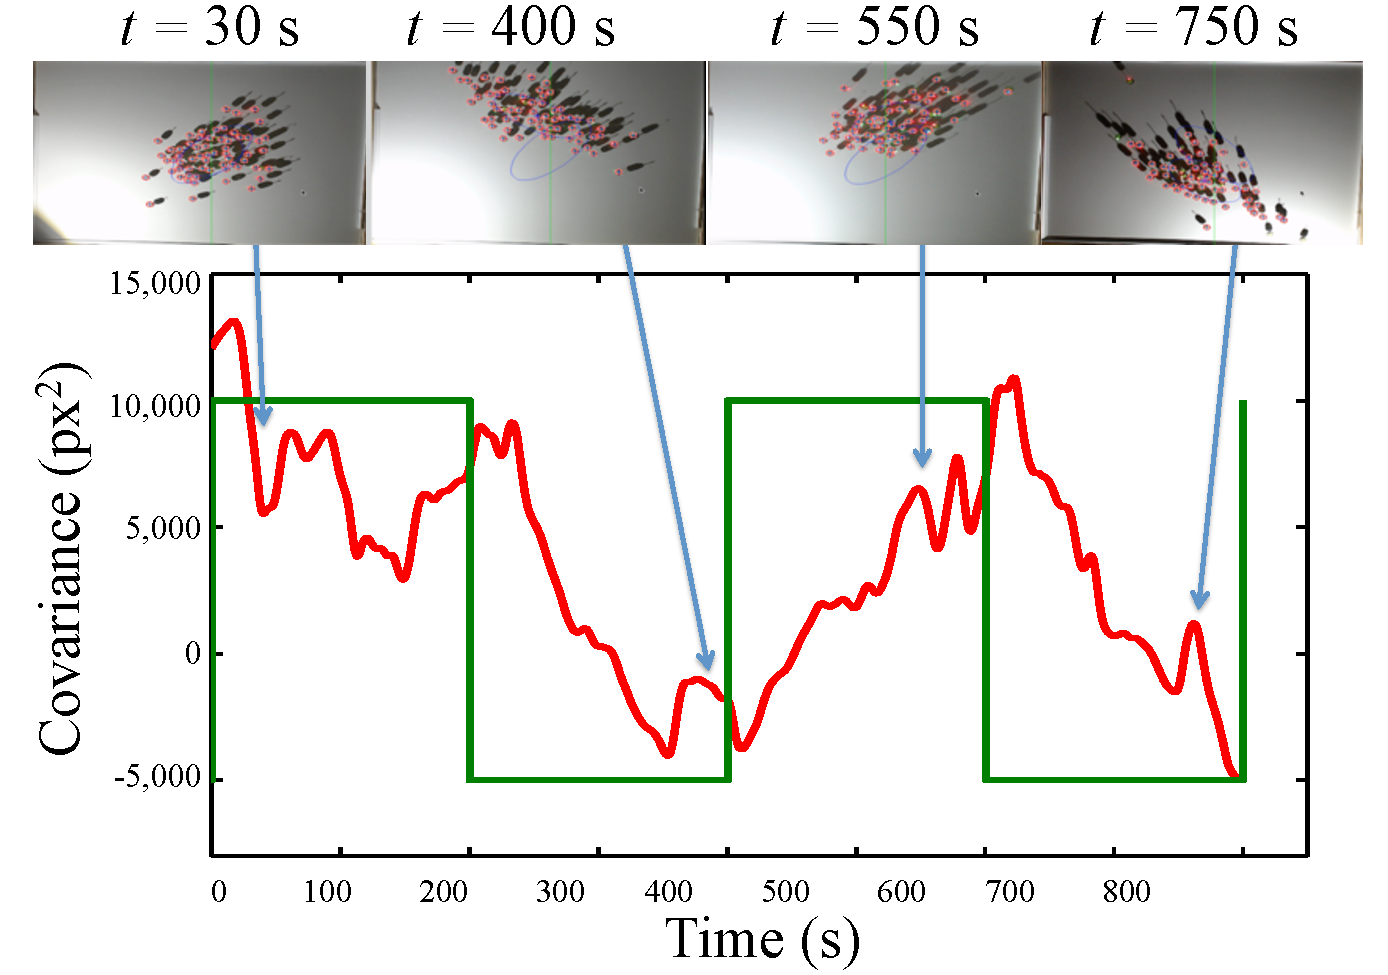
\includegraphics[width=\columnwidth]{experiment.pdf}
\end{center}
\caption{\label{fig:covExperiment}
Hardware demonstration steering 64 kilobot robots to desired covariance.  Frames above the plot show output from machine vision system and an overlaid covariance ellipse.
}
\end{figure}

